\documentclass[12pt]{article}
\usepackage[utf8]{inputenc}
\usepackage{polski}
\usepackage{graphicx}
\usepackage{amsmath}
\usepackage{bm}
\usepackage[table]{xcolor}
\usepackage[margin=2.5cm]{geometry}
\usepackage{anyfontsize}
\usepackage{caption}
\usepackage{rotating}
\graphicspath{ {img/} }

\begin{document}
	\begin{titlepage}
		\begin{flushright}
			\Huge DOKUMENTACJA TECHNICZNA
		\end{flushright}
		\hrulefill
		\vspace*{4cm}
		\centering
		
		LABORATORIUM INTERFEJSÓW OBIEKTOWYCH
		\vspace*{0.5cm}
		
		{\fontsize{64}{1.2}\selectfont \textbf{Amperomierz}}
		
		\vspace*{4cm}
		\underline{\normalsize AUTORZY:} \\
		\Large Tomasz \textbf{Masłoń} \\
		\Large Kamil \textbf{Nawrot}
		
		\vspace*{0.5cm}
		
		\underline{\normalsize OPIEKUN:} \\
		\Large mgr inż. Paweł \textbf{Dobrowolski}
		
		\vspace*{\fill}
		
\includegraphics[scale=0.3]{logo.png} \\
		{\footnotesize Wrocław, 2019}
	\end{titlepage}

\newpage

\tableofcontents
\listoffigures
\listoftables

\newpage

\section{Ogólny opis układu}
Realizowany układ elektroniczny miał za zadanie działać jako miernik natężenia prądu stałego z zakresu \textbf{0.1 - 2A}, przetwarzając podawany mu prąd na dwa standardy najczęściej stosowane w przemyśle:
\begin{itemize}
	\item sygnał napięciowy \textbf{0\,\dots10V}
	\item sygnał prądowy \textbf{4\,\dots20mA}
\end{itemize}
Oprócz tego, z wykorzystaniem przetwornika analogowo-cyfrowego \textbf{ICL7107}, zaimplementowano możliwość wyświetlania mierzonej wartości na trzech wyświetlaczach siedmiosegmentowych. Układ oparty został przede wszystkim na wzmacniaczach operacyjnych, które, skalując i przesuwając, przetwarzały sygnał wejściowy do odpowiednich wartości. \\

\section{Założenia projektowe}
\subsection{Zasilanie}
Układ należało zasilić symetrycznym napięciem $\pm$\textbf{12V}, ponieważ zastosowane wzmacniacze operacyjne również wymagają tego typu zasilenia. Konieczne było wyprowadzenie z generatorów trzech sygnałów: napięcia dodatniego, ujemnego oraz odniesienia (0V). 
\subsection{Przetwarzanie wartości mierzonej}
Sygnał mierzony musi być podawany na rezystor pomiarowy $\mathbf{0.1\Omega}$, aby uzyskać znany spadek napięcia, na którym mogą pracować kolejne elementy układu. Konieczna jest odpowiednia polaryzacja. Napięcie z rezystora podawane jest na kolejne wzmacniacze operacyjne, które działają w konfiguracji wzmacniacza nieodwracającego (przeskalowywanie sygnału) lub sumującego albo odejmującego (przesuwanie sygnału o stałą wartość). 
\subsection{Dokładność}
W całym urządzeniu stosowano rezystory z szeregu E24, które charakteryzują się tolerancją rzędu $\pm$5\%. Ich wartości bezpośrednio wpływają na parametr wzmocnienia każdego wzmacniacza oraz mnożniki dzielników napięciowych, w związku z czym w układzie mogą pojawiać się zauważalne różnice pomiędzy wartościami rzeczywistymi a przetworzonymi. W celu redukcji tych błędów, w koniecznych miejscach zastosowano precyzyjne potencjometry, które pozwalają na doregulowanie wartości napięcia. Przy takim rozwiązaniu powinno być możliwe uzyskanie dokładności pomiarów na poziomie 2\%. \\

\section{Koncepcja działania}\label{sec:koncepcja}
\subsection{Sygnał napięciowy 0\,\dots\,10V}\label{subsec:0-10V}
Mierzony prąd podawany jest na opornik pomiarowy. Spadek napięcia na nim może wynosić od 0.01V do 0.2V. Napięcie to kierowane jest na wzmacniacz różnicowy o pięćdziesięciokrotnym wzmocnieniu, zatem na jego wyjściu uzyskuje się napięcie \textbf{0.5-10V}. Kolejnym krokiem jest przesunięcie napięcia w dół o 0.5V z jednoczesnym wzmocnieniem, tak aby uzyskać zakres \textbf{0-10V}. Wzmacniacz realizujący tę operację pracuje w konfiguracji wzmacniacza odejmującego. Stałe napięcie 0.5V pobierane jest ze stabilizowanego zasilania sterownika \textbf{ICL7107} (opisanego w dalszej cześci dokumentacji). Wzmocnienie wynosi około $1.06$, tak aby podnieść górną granicę zakresu z 9.5 na 10V. Tak przetworzony sygnał wyprowadzony jest na złącze, które umożliwia jego pomiar.
\subsection{Sygnał prądowy 4\,\dots\,20mA}\label{subsec:4-20mA}
Napięcie uzyskane na poprzednim wzmacniaczu (0-10V) jest wykorzystywane w celu dalszego przetworzenia. Najpierw, za pomocą dzielnika napięciowego obniża się jego wartość do zakresu \textbf{0-4V}. Analogicznie jak 0.5V uzyskuje się napięcie 1V, które następnie jest dodawane za pomocą wzmacniacza sumującego o wzmocnieniu $1$ do sygnału z poprzedniego wzmacniacza operacyjnego. W ten sposób uzyskuje się wyjściowe napięcie o zakresie \textbf{1-5V}.
\subsection{Wyświetlacze siedmiosegmentowe}\label{subsec:7segmentowe}
Sygnał uzyskany za pierwszym wzmacniaczem operacyjnym układu (omówionym w punkcie \ref{subsec:0-10V}) jest kierowany na kolejny wzmacniacz o odwrotnym wzmocnieniu, który sprowadza sygnał ponownie do zakresu \textbf{0.01 - 0.2V}. Takie napięcie kierowane jest na sterownik wyświetlacza ($V_{in}$). Wymaga on także napięcia odniesienia $V_{ref}$ o wartości 1V, które także zostało uzyskane już wcześniej (punkt \ref{subsec:4-20mA}). ICL7107 wyświetla wartość napięcia uzyskaną ze wzoru:
\begin{equation*}
V_{disp} = 1000 \cdot \frac{V_{in}}{V_{ref}},
\end{equation*}
czyli wartości z zakresu \textbf{010 - 200}.
Koncepcję działania układu przedstawia także schemat blokowy, Załącznik do dokumentacji.

\section{Realizacja zasilania i jego zabezpieczenia}
\subsection{Główne zasilanie układu}
Cały układ zasilany jest stałym napięciem symetrycznym $\pm$12V. Układ połączenia zasilaczy (\textit{rys}) generuje potencjał odniesienia oraz dwie linie o potencjałach +12V i -12V względem masy. Na układ wyprowadzone są więc trzy osobne linie. Szeregowo z napięciem dodatnim połączona jest dioda Schottky'ego \textbf{BAT42}, która zabezpiecza układ przed odwrotnym podłączeniem zasilania. Działa ona analogicznie do zwykłej diody prostowniczej, jednak spadek napięcia na samym elemencie jest dużo niższy (około 0.3V).
\begin{figure}[h]
\centering
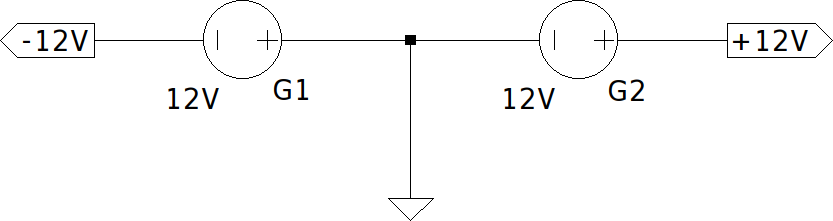
\includegraphics[scale=0.45]{power_supply.png}
\label{main_power_supply}
\caption{Ideowy schemat realizacji głównego zasilania układu}
\end{figure}

\subsection{Zasilanie przetwornika ICL7107}
Sterownik do obsługi wyświetlaczy wymaga zasilania symetrycznego o napięciu 5V. Uzyskuje się je z zasilania głównego z wykorzystaniem diód Zenera o napięciu przebicia równym 5.1V (\textit{rys}). Uzyskiwany w ten sposób spadek napięcia jest stabilny i niezależny od zmian wartości zasilania głównego. Fakt ten wykorzystuje się, używając napięcie zasilające ICL7107 także do uzyskiwania wartości 0.5V i 1V, które potrzebne są przy przesuwaniu zakresów napięcia na wzmacniaczach operacyjnych. Sygnał zasilający jest dodatkowo odfiltrowywany przez kondensatory elektrolityczne 10$\mu$F.
\begin{figure}[h]
\centering
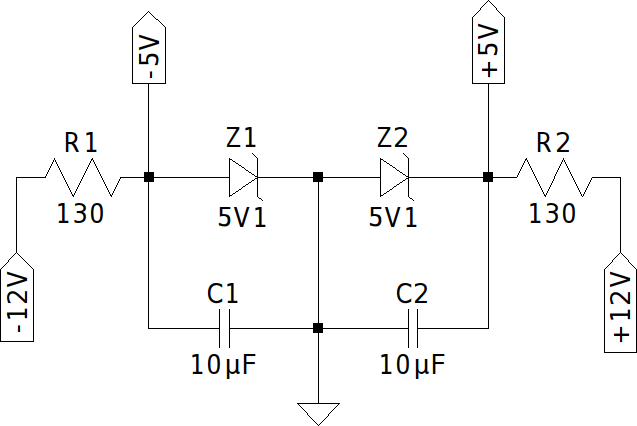
\includegraphics[scale=0.5]{icl_power_supply.png}
\label{icl_power_supply}
\caption{Ideowy schemat realizacji zasilania układu ICL7107}
\end{figure}

\subsection{Zasilanie diód wyświelaczy}
Przyjęto pobór prądu dla każdej czerwonej diody na poziomie 3-4mA. Realizację układu zasilającego przeprowadzono analogicznie jak przy sterowniku (\textit{rys}). Osobne zasilanie zapewnia stabilność zasilania ICL7107 oraz wyjść wtórników napięciowych utrzymujących napięcia 0.5V i 1V, ponieważ pobór prądu przy dużej ilości zapalonych segmentów może być znaczny i mógłby wpływać na inne elementy układu, gdyby zostało wykonane wspólne zasilanie. \\

\section{Testy układu}
\subsection{Badanie dokładności pomiarów na wyjściu napięciowym}
Przeprowadzono testy pomiarowe wyjścia napięciowego, podając mu wartości natężenia mierzone multimetrem \textbf{MXD-4660A}. Wykreślono także charakterystykę w celu sprawdzenia liniowości uzyskiwanych wyników. \\

\begin{minipage}[c]{0.3\textwidth}
\centering
\begin{tabular}{|c|c|}
\hline
		\cellcolor[gray]{0.9}$I [A]$ & \cellcolor[gray]{0.9}$U_{pom} [V]$ \\
		\hline
		0.100 & 0.012 \\
		\hline
		0.234 & 0.711 \\
		\hline
		0.388 & 1.505 \\
		\hline
		0.484 & 2.006 \\
		\hline
		0.589 & 2.556 \\
		\hline
		0.714 & 3.207 \\
		\hline
		0.829 & 3.802 \\
		\hline
		0.923 & 4.289 \\
		\hline
		1.049 & 4.952 \\
		\hline
		1.143 & 5.442 \\
		\hline
		1.291 & 6.211 \\
		\hline
		1.408 & 6.884 \\
		\hline
		1.500 & 7.308 \\
		\hline 
		1.654 & 8.120 \\
		\hline
		1.728 & 8.511 \\
		\hline
		1.855 & 9.204 \\
		\hline
		1.999 & 9.983 \\
		\hline
\end{tabular}
\captionof{table}{Wyniki pomiarów dla wyjścia napięciowego}
\end{minipage}
\begin{minipage}[c]{0.6\textwidth}
	\centering
	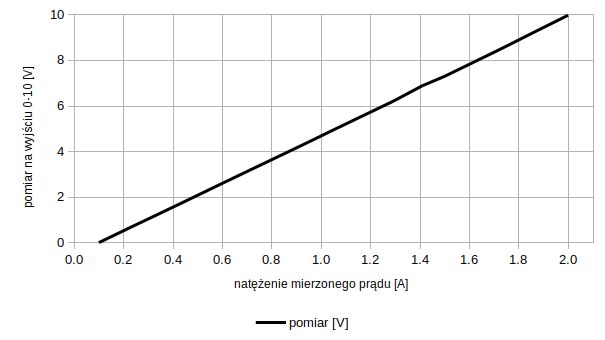
\includegraphics[width=\textwidth]{v_graph.png}
	\captionof{figure}{Wykres zależności wyjścia napięciowego od prądu mierzonego}
\end{minipage} \\ \\ \\

\noindent Maksymalne błędy uzyskanych w pomiarach wartości oscylują w granicach 2-2.5\%. Uzyskana charakterystyka jest, zgodnie z założeniami, niemal idealnie liniowa.

\subsection{Badanie dokładności pomiarów na wyjściu prądowym}
Analogicznie zbadano wyjście prądowe 4-20mA i wykreślono charakterystykę zależności prądu mierzonego i wyjściowego. Błędu względne rzadko i nieznacznie przekraczały 1\%, natomiast kształt uzyskanej charakterystyki także był liniowy.

\begin{minipage}[c]{0.3\textwidth}
\centering
\begin{tabular}{|c|c|}
\hline
		\cellcolor[gray]{0.9}$I [A]$ & \cellcolor[gray]{0.9}$I_{pom} [mA]$ \\
		\hline
		0.103 & 4.023 \\
		\hline
		0.211 & 4.921 \\
		\hline
		0.335 & 5.979 \\
		\hline
		0.406 & 6.579 \\
		\hline
		0.514 & 7.509 \\
		\hline
		0.613 & 8.349 \\
		\hline
		0.710 & 9.176 \\
		\hline
		0.810 & 10.029 \\
		\hline
		0.935 & 11.096 \\
		\hline
		1.053 & 12.113 \\
		\hline
		1.107 & 12.575 \\
		\hline
		1.195 & 13.328 \\
		\hline
		1.329 & 14.461 \\
		\hline 
		1.429 & 15.341 \\
		\hline
		1.502 & 15.976 \\
		\hline
		1.619 & 16.991 \\
		\hline
		1.714 & 17.812 \\
		\hline
		1.853 & 19.025 \\
		\hline
		2.000 & 20.230 \\
		\hline
\end{tabular}
\captionof{table}{Wyniki pomiarów dla wyjścia prądowego}
\end{minipage}
\begin{minipage}[c]{0.6\textwidth}
	\centering
	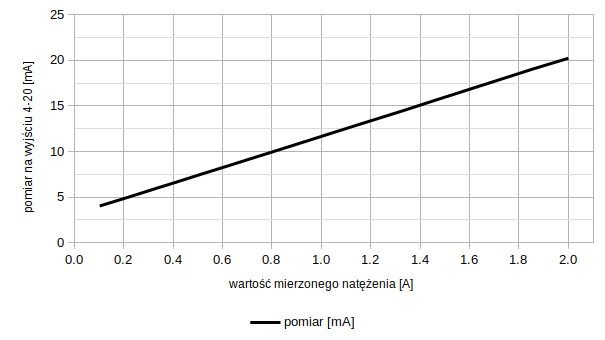
\includegraphics[width=\textwidth]{i_graph.png}
	\captionof{figure}{Wykres zależności wyjścia prądowego od prądu mierzonego}
\end{minipage}

\subsection{Sprawdzanie obciążności wyjścia prądowego}
Zbadano także parametr obciążności wyjścia prądowego poprzez podłączenie opornicy dekadowej szeregowo z wyjściem. Następnie stopniowo zwiększano rezystancję, obserwując stabilność prądu na wyjściu. Wyznaczono rezystancję graniczną, przy której prąd zaczyna znacząco spadać dla pomiaru 0.1A, 1.05A i 2.0A.
\begin{equation*}
R_{gran(0.10A)} = 2600\Omega
\end{equation*}

\begin{equation*}
R_{gran(1.05A)} = 740\Omega
\end{equation*}

\begin{equation*}
R_{gran(2.00A)} = 345\Omega
\end{equation*} \\

\noindent Minimalna obciążność dla maksymalnego natężenia prądu mierzonego spełniła założenia projektowe i oczekiwania względem tego parametru..

\begin{figure}
	\centering
	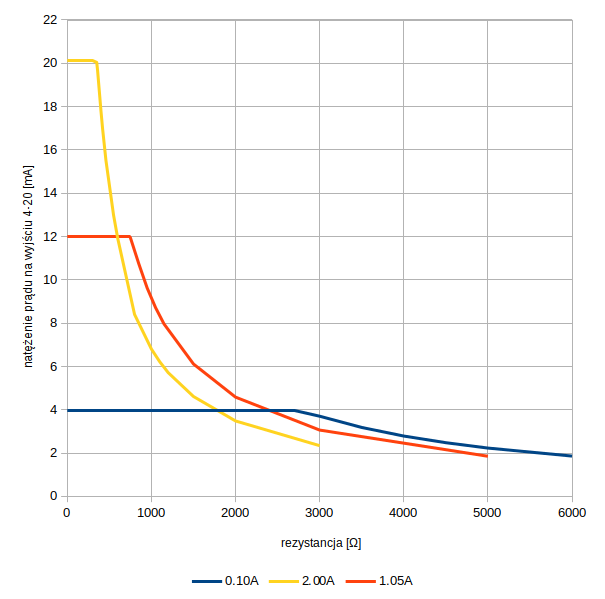
\includegraphics[scale=1]{r_graph.png}
	\caption{Pomiar obciążności dla trzech różnych wartości natężenia mierzonego}
\end{figure}

\section{Zastosowane elementy i układy elektroniczne}
\subsection{Układy scalone}
\begin{itemize}
	\item wzmacniacz operacyjny \textbf{TL081CP} (\textit{x8}) - przetwarzanie zakresów napięcia, wtórniki napięciowe
	\begin{figure}[h]
	\centering
	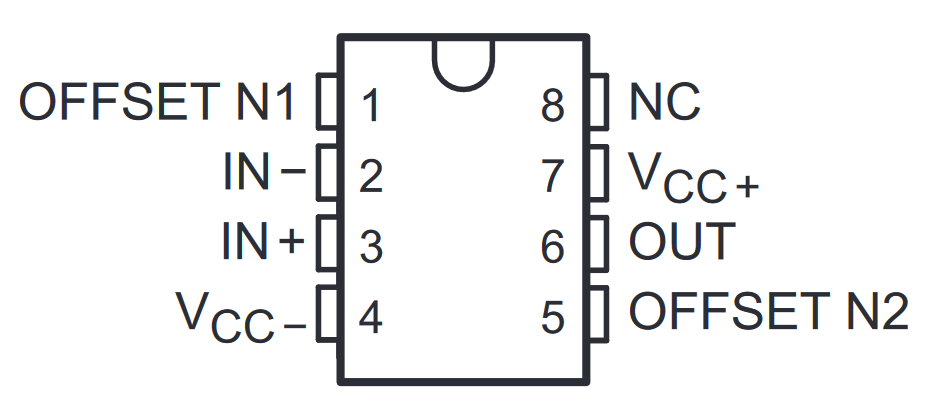
\includegraphics[scale=0.2]{tl081_pinout.png}
	\label{tl081_pinout}
	\caption{Konfiguracja pinów wzmacniacza operacyjnego TL081}
	\end{figure}
	\item przetwornik analogowo-cyfrowy \textbf{ICL7107} - przetwarzanie analogowego sygnału napięciowego na 		cyfrowe sterowanie trzema wyświetlaczami siedmiosegmentowymi
	\begin{figure}[h]
	\centering
	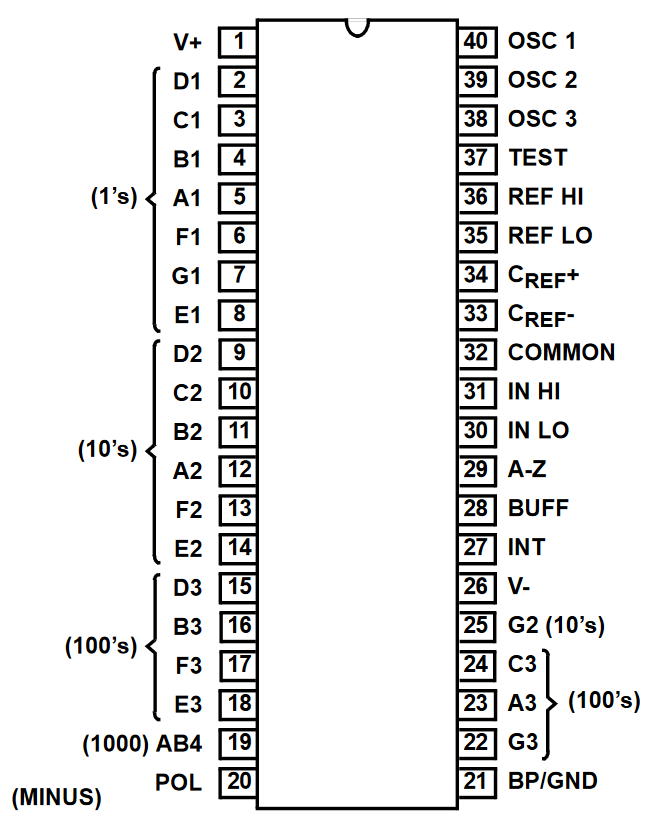
\includegraphics[scale=0.3]{icl7107_pinout.png}
	\label{icl7107_pinout}
	\caption{Konfiguracja pinów przetwornika A/C ICL7107}
	\end{figure}
\end{itemize}
\subsection{Elementy półprzewodnikowe}
\begin{itemize}
	\item tranzystor bipolarny typu NPN \textbf{BD139}
	\item dioda Schottky'ego \textbf{BAT42} - zabezpieczenie głównego zasilania przed odwrotną polaryzacją
	\item dioda Zenera 5V1 (\textit{x2}) - stabilizator napięcia zasilającego przetwornik ICL7107
	\item dioda Zenera 5V6 - stabilizator napięcia zasilającego wyświetlacze
\end{itemize}
Wymieniono tylko układy i elementy o większym znaczeniu i bardziej skomplikowanym działaniu. Wykaz wszystkich użytych w projekcie elementów, wraz z podstawowymi parametrami, znajduje się w Załączniku dołączonym do dokumentacji.


\begin{sidewaysfigure}[H]
	\centering
	\LARGE \textbf{ZAŁĄCZNIK 1} \\
	\large Koncepcyjny schemat blokowy urządzenia \\
	\includegraphics[scale=0.90, origin=c]{diagram_blokowy.png}
\end{sidewaysfigure}
	

\begin{sidewaysfigure}[H]
	\centering
	\LARGE \textbf{ZAŁĄCZNIK 2} \\
	\large Schemat symulacyjny układu 
	\includegraphics[scale=0.82, origin=c]{ammeter.png}
\end{sidewaysfigure}

\newpage
\begin{center}
\LARGE \textbf{ZAŁĄCZNIK 3} \\
\large Wykaz elementów i układów wykorzystanych w projekcie \\
\end{center}

\begin{minipage}[c]{0.45\linewidth}
\tiny
\centering
\begin{tabular}{|c|c|c|}
\hline
element & wartość & opis \\
\hline
C1 & 10$\mu$F & kondensator elektrolityczny \\
\hline
C2 & 10$\mu$F & kondensator elektrolityczny \\
\hline
C3 & 100$p$F & kondensator ceramiczny \\
\hline
C4 & 0.1$\mu$F & kondensator ceramiczny \\
\hline
C5 & 0.047$\mu$F & kondensator ceramiczny \\
\hline
C6 & 0.22$\mu$F & kondensator ceramiczny \\
\hline
C7 & 0.01$\mu$F & kondensator ceramiczny \\
\hline
C8 & 10$\mu$F & kondensator ceramiczny \\
\hline
D1 & 5V1 & dioda Zenera \\
\hline
D2 & 5V1 & dioda Zenera \\
\hline
D3 & BAT42 & dioda Schottky'ego 200mA/30V \\
\hline
D4 & 5V6 & dioda Zenera \\
\hline
DIS1 & 7SEG-CA & wyświetlacz 7-segmentowy FJ5161BH \\
\hline
DIS2 & 7SEG-CA & wyświetlacz 7-segmentowy FJ5161BH \\
\hline
DIS3 & 7SEG-CA & wyświetlacz 7-segmentowy FJ5161BH \\
\hline 
G1 & 12V & bateria/zasilacz \\
\hline
G2 & 12V & bateria/zasilacz \\
\hline 
IC1 & TL081P & wzmacniacz operacyjny \\
\hline 
IC2 & TL081P & wzmacniacz operacyjny \\
\hline 
IC3 & ICL7107 & przetwornik A/C \\
\hline 
IC4 & TL081P & wzmacniacz operacyjny \\
\hline
IC5 & TL081P & wzmacniacz operacyjny \\
\hline 
IC6 & TL081P & wzmacniacz operacyjny \\
\hline 
IC7 & TL081P & wzmacniacz operacyjny \\
\hline 
IC8 & TL081P & wzmacniacz operacyjny \\
\hline 
IC9 & TL081P & wzmacniacz operacyjny \\
\hline
R1 & 270 & rezystor 250mW \\
\hline
R2 & 270 & rezystor 250mW \\
\hline
R3 & 100 & rezystor 250mW \\
\hline
R4 & 50k & potencjometr precyzyjny 3296X \\
\hline
R5 & 4k7 & rezystor 250mW \\
\hline
R6 & 270 & rezystor 250mW \\
\hline
R7 & 270 & rezystor 250mW \\
\hline
R8 & 270 & rezystor 250mW \\
\hline
R9 & 1M & rezystor 250mW \\
\hline
R10 & 270 & rezystor 250mW \\
\hline
R11 & 100 & rezystor 250mW \\
\hline
R12 & 270 & rezystor 250mW \\
\hline
R13 & 100 & rezystor 250mW \\
\hline
R14 & 270 & rezystor 250mW \\
\hline
R15 & 4k7 & rezystor 250mW \\
\hline
R16 & 270 & rezystor 250mW \\
\hline
\end{tabular}
\end{minipage}
\begin{minipage}[t]{0.45\linewidth}
\tiny
\centering
\begin{tabular}{|c|c|c|}
\hline
element & wartość & opis \\
\hline
R17 & 100k & potencjometr precyzyjny 3296X \\
\hline
R18 & 20k & rezystor 250mW \\
\hline
R19 & 100k & rezystor 250mW \\
\hline
R20 & 470k & rezystor 250mW \\
\hline
R21 & 270 & rezystor 250mW \\
\hline
R22 & 270 & rezystor 250mW \\
\hline
R23 & 1M & rezystor 250mW \\
\hline
R24 & 270 & rezystor 250mW \\
\hline
R25 & 270 & rezystor 250mW \\
\hline
R26 & 270 & rezystor 250mW \\
\hline
R27 & 270 & rezystor 250mW \\
\hline
R28 & 270 & rezystor 250mW \\
\hline
R29 & 270 & rezystor 250mW \\
\hline
R30 & 270 & rezystor 250mW \\
\hline
R31 & 110 & rezystor 1W \\
\hline
R32 & 270 & rezystor 250mW \\
\hline
R33 & 1M & rezystor 250mW \\
\hline
R34 & 15k & rezystor 250mW \\
\hline
R35 & 10k & rezystor 250mW \\
\hline
R36 & 1M & rezystor 250mW \\
\hline
R37 & 0.1 & rezystor 5W \\
\hline
R38 & 300 & rezystor 250mW \\
\hline
R39 & 300 & rezystor 250mW \\
\hline
R40 & 560 & rezystor 250mW \\
\hline
R41 & 560 & rezystor 250mW \\
\hline
R42 & 560 & rezystor 250mW \\
\hline
R43 & 15k & rezystor 250mW \\
\hline
R44 & 15k & rezystor 250mW \\
\hline
R45 & 560 & rezystor 250mW \\
\hline
R46 & 15k & rezystor 250mW \\
\hline
R47 & 15k & rezystor 250mW \\
\hline
R48 & 15k & rezystor 250mW \\
\hline
R49 & 15k & rezystor 250mW \\
\hline
R50 & 5k & potencjometr precyzyjny 3296X \\
\hline
R51 & 16k & rezystor 250mW \\
\hline
R52 & 20k & potencjometr precyzyjny 3296X \\
\hline
R53 & 300 & rezystor 250mW \\
\hline
R54 & 2k & potencjometr precyzyjny 3296X \\
\hline
R55 & 500 & potencjometr precyzyjny 3296X \\
\hline
SJ1 & - & zwora \\
\hline
T1 & BD139 & tranzystor typu NPN \\
\hline
 &  &  \\
\hline
\end{tabular}
\end{minipage}

\end{document}